\documentclass[8pt]{extarticle}
\title{}
\author{Avinash Iyer}
\date{}

%font setup
%
%\usepackage[math]{anttor}

\usepackage{newpxtext,eulerpx}
%paper setup
\usepackage{geometry}
\geometry{letterpaper, portrait, margin=1in}
\usepackage{fancyhdr}

%symbols
\usepackage{blkarray}
\usepackage{nicematrix}
\usepackage{amsmath}
\usepackage{amssymb}
\usepackage{hyperref}
\usepackage{gensymb}

\usepackage[T1]{fontenc}
\usepackage[utf8]{inputenc}

%chemistry stuff
\usepackage[version=4]{mhchem}
\usepackage{chemfig}

%plotting
\usepackage{pgfplots}
\usepackage{tikz}

%\usepackage{natbib}

%graphics stuff
\usepackage{graphicx}
\graphicspath{ {./images/} }

%code stuff
%when using minted, make sure to add the -shell-escape flag
%you can use lstlisting if you don't want to use minted
%\usepackage{minted}
%\usemintedstyle{pastie}
%\newminted[javacode]{java}{frame=lines,framesep=2mm,linenos=true,fontsize=\footnotesize,tabsize=3,autogobble,}
%\newminted[cppcode]{cpp}{frame=lines,framesep=2mm,linenos=true,fontsize=\footnotesize,tabsize=3,autogobble,}

\usepackage{listings}
\usepackage{color}
\definecolor{dkgreen}{rgb}{0,0.6,0}
\definecolor{gray}{rgb}{0.5,0.5,0.5}
\definecolor{mauve}{rgb}{0.58,0,0.82}

\lstset{frame=tb,
	language=Java,
	aboveskip=3mm,
	belowskip=3mm,
	showstringspaces=false,
	columns=flexible,
	basicstyle={\small\ttfamily},
	numbers=none,
	numberstyle=\tiny\color{gray},
	keywordstyle=\color{blue},
	commentstyle=\color{dkgreen},
	stringstyle=\color{mauve},
	breaklines=true,
	breakatwhitespace=true,
	tabsize=3
}
% text + color boxes
\usepackage{tcolorbox}
\newtcolorbox{mathbox}[1]{colback = white, title = {#1}}
\pagestyle{fancy}
\fancyhf{}
\rhead{Avinash Iyer}
\lhead{Homework Section 1.1, Individual}
\begin{document}
\begin{mathbox}{Problem 1.1.1}
    Determine which bipartite graphs are complete graphs
    \tcblower
 The graph $K_{1,1}$ is the only bipartite graph that is complete.
\end{mathbox}
\begin{mathbox}{Problem 1.1.3}
    Using rectangular blocks whose entries are equal, write down an adjacency matrix for $K_{m,n}$
    \tcblower
  \[
    K_{m,n} = \begin{bNiceMatrix}[first-row,first-col]
          & a_1 & a_2 & \cdots & a_m & b_1 & b_2 & \cdots & b_n \\
      a_1 & 0 & 0 & \cdots & 0 & 1 & 1 & \cdots & 1 \\
      a_2 & 0 & 0 & \cdots & 0 & 1 & 1 & \cdots & 1 \\
      \vdots & \vdots & \vdots & \ddots & \vdots & \vdots & \ddots & \vdots \\
      a_m & 0 & 0 & \cdots & 0 & 1 & 1 & \cdots & 1 \\
      b_1 & 1 & 1 & \cdots & 1 & 0 & 0 & \cdots & 0 \\
      b_2 & 1 & 1 & \cdots & 1 & 0 & 0 & \cdots & 0 \\
      \vdots & \vdots & \vdots & \ddots & \vdots & \vdots & \ddots & \vdots \\
      b_n & 1 & 1 & \cdots & 1 & 0 & 0 & \cdots & 0 \\
    \end{bNiceMatrix}
  \]
  \end{mathbox}
\begin{mathbox}{Problem 1.1.5}
    Prove or disprove: If every vertex of a simple graph $G$ has degree 2, then $G$ is a cycle.
    \tcblower

  Let $G$ be the following graph:
    \begin{center}
        \begin{tikzpicture}
          \draw[fill = black] (1,1) circle (3pt);
          \draw[fill = black] (1,-1) circle (3pt);
          \draw[fill = black] (2,0) circle (3pt);

          \draw[fill = black] (-2,0) circle (3pt);
          \draw[fill = black] (-1,1) circle (3pt);
          \draw[fill = black] (-1,-1) circle (3pt);

        \draw[thick] (1,1) -- (1,-1) -- (2,0) -- (1,1);
        \draw[thick] (-1,1) -- (-1,-1) -- (-2,0) -- (-1,1);
        \end{tikzpicture}
    \end{center}
    Every vertex in $G$ has a degree 2, yet $G$ is not a cycle. 
  \end{mathbox}
  \pagebreak
\begin{mathbox}{Problem 1.1.8}
    Prove that the 8 vertex graph below decomposes into copies of $K_{1,3}$ and also into copies of $P_4$
  \begin{center}
      \begin{tikzpicture}
        \draw[fill=black] (1,1) circle (3pt);
        \draw[fill=black] (-1,1) circle (3pt);
        \draw[fill=black] (-1,-1) circle (3pt);
        \draw[fill=black] (1,-1) circle (3pt);

        \draw[fill=black] (2,2) circle (3pt);
        \draw[fill=black] (-2,2) circle (3pt);
        \draw[fill=black] (-2,-2) circle (3pt);
        \draw[fill=black] (2,-2) circle (3pt);
        
        \draw[thick] (1,1) -- (-1,1) -- (-1,-1) -- (1,-1) -- (1,1);
        \draw[thick] (2,2) -- (-2,2) -- (-2,-2) -- (2,-2) -- (2,2);
        \draw[thick] (1,1) -- (2,2);
        \draw[thick] (-1,1) -- (-2,2);
        \draw[thick] (-1,-1) -- (-2,-2);
        \draw[thick] (1,-1) -- (2,-2);
      \end{tikzpicture}
  \end{center} 
\tcblower
    \begin{center}
      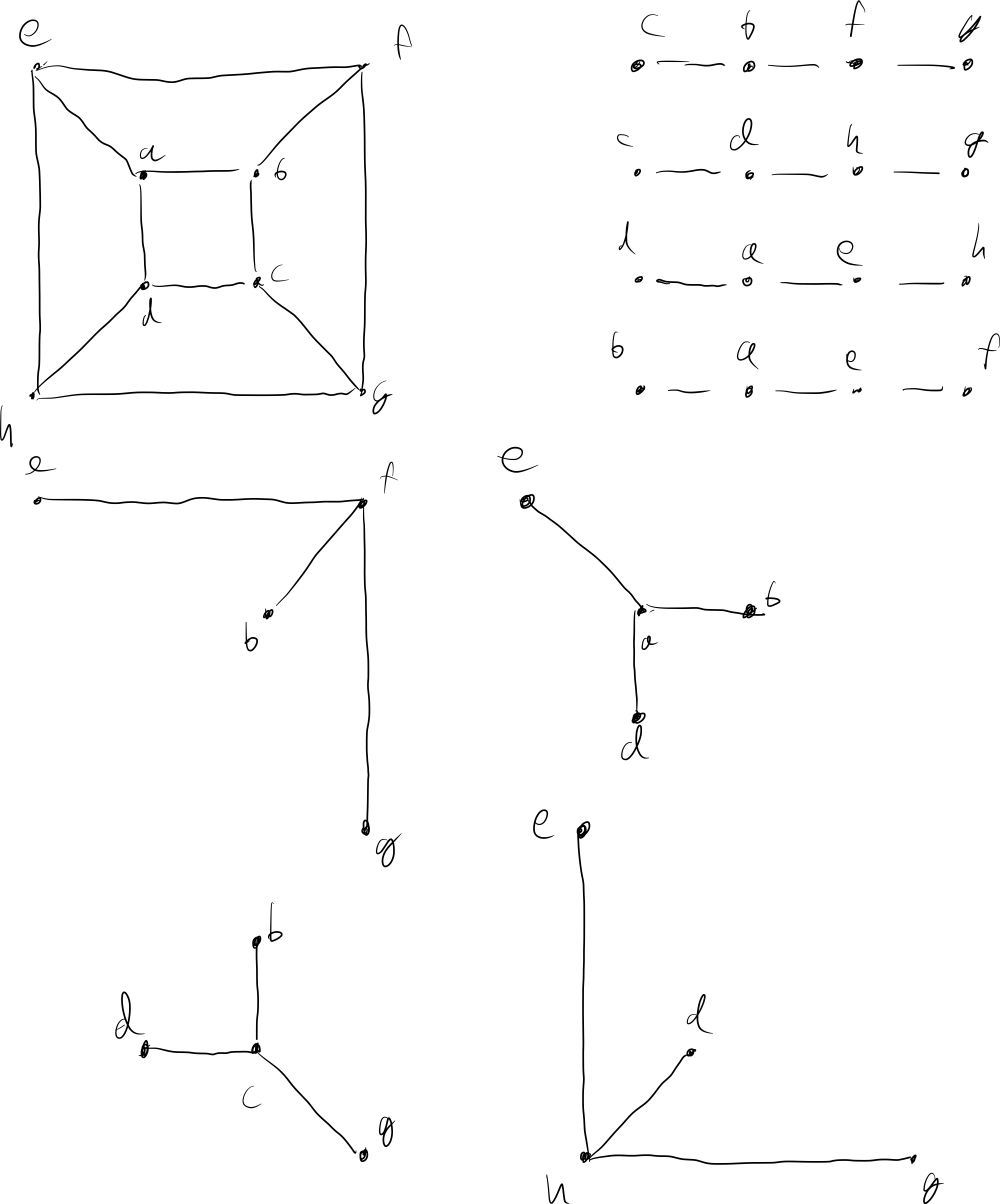
\includegraphics[width=10cm]{1_1_8}
    \end{center}
  \end{mathbox}
    \pagebreak
  \begin{mathbox}{Problem 1.1.9}
      Prove that the graph below is isomorphic to the complement of the previous graph
  \begin{center}
      \begin{tikzpicture}
        \draw[fill=black] (1,1) circle (3pt);
        \draw[fill=black] (-1,1) circle (3pt);
        \draw[fill=black] (-1,-1) circle (3pt);
        \draw[fill=black] (1,-1) circle (3pt);

        \draw[fill=black] (2,2) circle (3pt);
        \draw[fill=black] (-2,2) circle (3pt);
        \draw[fill=black] (-2,-2) circle (3pt);
        \draw[fill=black] (2,-2) circle (3pt);
        
        \draw[thick] (1,1) -- (-1,1) -- (-1,-1) -- (1,-1) -- (1,1);
        \draw[thick] (2,2) -- (-2,2) -- (-2,-2) -- (2,-2) -- (2,2);
        \draw[thick] (1,1) -- (2,2);
        \draw[thick] (-1,1) -- (-2,2);
        \draw[thick] (-1,-1) -- (-2,-2);
        \draw[thick] (1,-1) -- (2,-2);
        \draw[thick] (2,2) -- (1,-1);
        \draw[thick] (2,-2) -- (1,1);
        \draw[thick] (-2,2) -- (-1,-1);
        \draw[thick] (-2,-2) -- (-1,1);
      \end{tikzpicture}
  \end{center} 
      \tcblower
  \begin{center}
    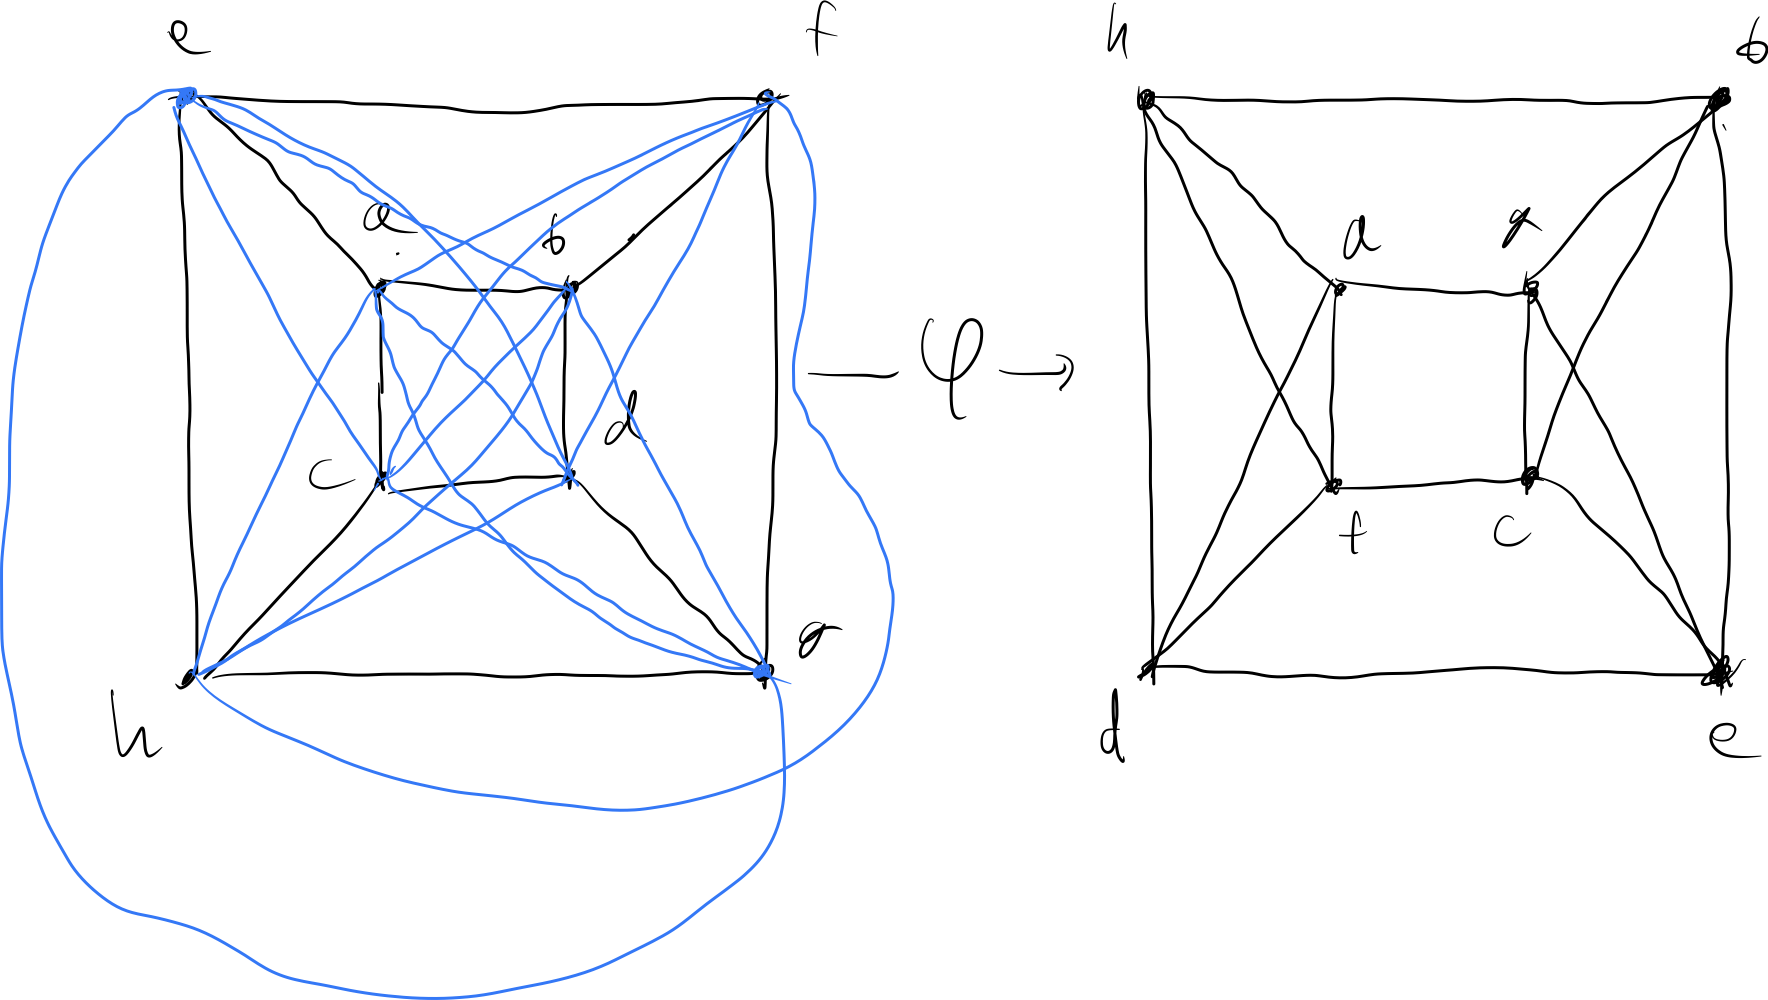
\includegraphics[width=10cm]{1_1_9}
  \end{center}
    \end{mathbox}
  \begin{mathbox}{Problem 1.1.10}
       Prove or disprove: the complement of a simple disconnected graph must be connected.
       \tcblower

   Let $G$ be a graph that is disconnected. We want to show that $\forall x,y\in V(G), \exists x,z$ path. We can split into two cases.
     \begin{itemize}
       \item Suppose $x\not\leftrightarrow y$ in $G$. Then, in $\overline{G}$, $x\leftrightarrow y$ by the definition of a graph complement.
       \item Suppose $x\leftrightarrow y$ in $G$. Then, since $G$ is disconnected, we know that there must be some $z\in V(G)$ such that there is no $x,z$ path. Since there is no $x,z$ path, then there is no $y,z$ path. In particular, this means $x\not\leftrightarrow z$ and $y\not\leftrightarrow z$ in $G$. Therefore, in $\overline{G}$, we have that $x\leftrightarrow z$ and $y\leftrightarrow z$, meaning there is a path between $x$ and $y$.
     \end{itemize}
     \end{mathbox} 
\end{document}
